%!TEX program = xelatex
% 完整编译: xelatex -> biber/bibtex -> xelatex -> xelatex
\documentclass[lang=cn,a4paper,founder,bibend=bibtex,citestyle=gb7714-2015, bibstyle=gb7714-2015]{elegantpaper}
\ExecuteBibliographyOptions{sorting=gb7714-2015}
\usepackage{listings}
\title{人工智能软件开发与实践大作业 技术报告} % 标题
\author{lkyu} % 作者
\institute{} % 机构

\version{} % 版本,可不写(删去本行)

\date{\zhdate{2024/09/08}} % 日期

% 本文档命令
\usepackage{array}
\usepackage{float} % 使图片表格支持精确位置
\newcommand{\ccr}[1]{\makecell{{\color{#1}\rule{1cm}{1cm}}}}
\addbibresource[location=local]{reference.bib} % 参考文献,不要删除

\begin{document}

\maketitle

\begin{abstract} % 摘要

	在当前人工智能技术的快速发展背景下,聊天机器人作为一种新兴的交互方式,正逐渐渗透到人们的日常生活中。本项目旨在开发一个集成文档问答和角色扮演功能的人工智能聊天机器人。项目的核心目标是提供一个用户友好的界面,通过自然语言处理技术实现高效的信息检索和交互体验。

	为了实现这一目标,项目采用了gradio库来构建可视化前端界面,使得用户能够直观地与聊天机器人进行互动。在后端,项目集成了百度千帆的“ernie-speed-128k”大型语言模型(LLM)和huggingface上的“BAAI/bge-small-zh”开源嵌入模型,以支持文档阅读和问答功能。通过调用这些模型,聊天机器人能够理解和处理用户上传的长文本文件,提供准确的信息检索和问答服务。此外,项目还实现了一个角色扮演聊天机器人,它能够记住对话历史并根据预设的角色人设进行互动。
	\keywords{大模型;文本生成;文档阅读;角色扮演聊天} % 关键词
\end{abstract}

\section{项目概述} % 章节

在人工智能技术日益成熟的今天,聊天机器人作为人机交互的重要方式之一,其应用范围和功能复杂性都在不断扩展\cite{konstantin_barabanov_zafar_jafarov_zafar_jafarov_2024}。本项目“人工智能软件开发与实践大作业展示”旨在开发一个多功能的人工智能聊天机器人,该机器人不仅能够进行文档问答,还能进行角色扮演,以提供更丰富的用户体验。项目的通过结合先进的自然语言处理技术和机器学习模型,实现了一个能够理解和响应用户需求的智能系统。

项目的创建并实现了两个主要功能:文档问答聊天机器人和角色扮演聊天机器人。文档问答聊天机器人利用百度千帆的“ernie-speed-128k”大型语言模型和huggingface上的“BAAI/bge-small-zh”嵌入模型,能够处理和理解用户上传的文档内容,提供准确的信息检索和问答服务。这一功能特别适合需要处理大量文本数据的场景,如法律咨询、学术研究等。

角色扮演聊天机器人则通过维护对话历史记录,结合预设的角色人设,使得机器人能够在对话中模拟并保持特定角色的行为和语言风格。

为了使这些功能直观地体现在屏幕上,项目采用了gradio库来构建用户友好的可视化界面,用户可以通过简单的图形界面与机器人进行互动。

\section{技术架构}



\subsection{可视化前端界面} % 子章节

在本项目的实现中,技术架构是构建高效、用户友好的人工智能聊天机器人的关键。项目采用了Gradio库来创建可视化前端界面,该界面是用户与机器人交互的直接媒介,允许用户通过直观的方式提交问题并接收答案。Gradio是一个开源的Python库,专门用于创建机器学习模型的交互式界面,它支持快速原型设计、模型验证、演示和教学,非常适合于本项目的需要。

在项目的前端设计中,我们定义了两个主要的交互界面,分别用于角色扮演聊天和长文档阅读。角色扮演聊天界面允许用户与机器人进行基于预设角色的对话,而长文档阅读界面则允许用户上传文档并提出相关问题。这两个界面的设计充分利用了Gradio的功能,通过gr.Blocks()和gr.TabbedInterface来组织和展示不同的交互组件。

在角色扮演聊天界面中,我们使用了gr.Chatbot()组件来展示对话历史,并通过gr.Textbox()和gr.Button()组件来接收用户的输入和触发对话更新。

\begin{lstlisting}[language=python]
	with gr.Blocks() as app1:
		chatbot = gr.Chatbot()
		msg = gr.Textbox(label="输入")
		submit_btn = gr.Button("Submit")
		submit_btn.click(fn=update_chat, inputs=[chatbot, msg], outputs=[chatbot, msg])
		msg.submit(fn=update_chat, inputs=[chatbot, msg], outputs=[chatbot, msg])
		clear = gr.ClearButton([msg, chatbot])
\end{lstlisting}

在长文档阅读界面中,我们通过gr.Interface()组件来实现文件上传和文档内容的读取。用户可以上传文档,系统会调用后端的处理函数来读取和分析文档内容,然后返回相应的答案。

\begin{lstlisting}[language=python]
	with gr.Blocks() as app2:
		upload_interface = gr.Interface(fn=save_file, inputs="file", outputs="text")
		read_input = gr.Textbox(label="向文档提问")
		read_output = gr.Textbox(label="结果")
		read_interface = gr.Interface(fn=read, inputs=read_input, outputs=read_output)
\end{lstlisting}

\subsection{功能实现}

功能实现是构建人工智能聊天机器人的核心部分,涉及到文档问答和角色扮演两大功能。我们在调用千帆模型API完成文本生成任务的同时,辅以本地部署的开源文本向量模型,以更好的完成需求。

\subsubsection{文档问答聊天机器人} % 下一级子章节

文档问答聊天机器人 的实现基于百度千帆的“ernie-speed-128k”大型语言模型(LLM)和huggingface上的“BAAI/bge-small-zh”模型。这些模型提供了强大的文本理解和生成能力,使得机器人能够处理复杂的文档问答任务。通过使用langchain库,我们能够将文本转换为语义向量,进而实现高效的信息检索和问答。在后端,我们调用了read函数,该函数负责处理用户上传的文档,并返回相应的答案。例如,当用户上传一个文档并提出问题时,read函数会被触发,它首先通过TextLoader加载文档内容,然后使用RecursiveCharacterTextSplitter进行文本分割,最后通过Chroma向量数据库和create\_retrieval\_chain创建的检索链来找到答案。


\begin{lstlisting}[language=python]
	# 导入语料
    loader = TextLoader("./temp.txt")
    text = loader.load()

    # 导入文本
    documents = text_splitter.split_documents(text)

    # 存入向量数据库
    vector = Chroma.from_documents(documents, embeddings)
    retriever = vector.as_retriever()
    retrieval_chain = create_retrieval_chain(retriever, document_chain)
\end{lstlisting}

\begin{lstlisting}[language=python]
	def read(input_text):
		if loader is None:
			return "请上传纯文本语料!"
		else:
			return retrieval_chain.invoke({"input": input_text})["answer"]
\end{lstlisting}

\subsection{角色扮演聊天机器人}

角色扮演聊天机器人 的实现则侧重于对话管理和上下文理解。通过维护一个对话历史记录列表conversation\_history,机器人能够记住之前的对话内容,从而在角色扮演中提供连贯和合理的回答。我们使用了百度千帆的“ernie-speed-128k”模型来生成回答,该模型能够根据当前的对话历史和预设的角色人设来生成合适的回复。我们定义了send\_request函数,它负责发送用户输入到百度的API,并接收模型生成的回答。此外,我们还在main.py中定义了update\_chat函数,用于更新聊天记录并触发对话生成。

\section{功能实现细节}

\subsection{prompt优化}

在实现文档问答聊天机器人时,我们发现prompt的设置对于模型的效果至关重要。prompt可以帮助模型更好地理解用户的需求,从而更准确地生成答案。prompt的设置可以分为两种类型:固定prompt和可变prompt。固定prompt是指模型在生成答案时,始终使用固定的模板,我们的项目中使用的就是固定prompt。

在文档问答聊天机器人中,我们使用了如下的固定prompt模板,规范了LLM的生成效果:

\begin{lstlisting}[language=python,showstringspaces=false]
# 创建提示词模板
prompt = ChatPromptTemplate.from_template(
	"""
	使用下面的语料来回答本模板最末尾的问题。如果你不知道问题的答案,直接回答 "我不知道",禁止随意编造答案。
	为了保证答案尽可能简洁,你的回答必须不超过三句话,你的回答中不可以带有星号。
	以下是一对问题和答案的样例:
		请问:秦始皇的原名是什么
		秦始皇原名嬴政。

	以下是语料:
	<context>
	{context}
	</context>

	Question: {input}
	"""
)
\end{lstlisting}

角色扮演聊天机器人的prompt则负责初始化人设:

\begin{lstlisting}[language=python,]
	payload = json.dumps(
        {
            "messages": conversation_history,  # 发送对话历史记录
            "stream": False,
            "temperature": 0.9,
            "top_p": 0.7,
            "penalty_score": 1,
            "system": "现在我们开始一个角色扮演游戏,以下是你的人设:你是尼克·王尔德(Nick Wilde),男,是2016年迪士尼动画电影《疯狂动物城》中的男主角。原型是赤狐。原名尼古拉斯·皮比里厄斯·王尔德(Nicholas Piberius Wilde),在中国大陆地区又被称作狐尼克,由杰森·贝特曼和凯特·索西配音。你少时因遭遇挫折和他人的偏见,被迫放弃了自己的理想,打算不再为谁付出,长大后以坑蒙拐骗为生。你口若悬河、思维敏捷、谎技高超但却内心善良,同时拥有过目不忘的惊人记忆力。因为意外而和动物城警官朱迪·霍普斯被卷进了一个意欲颠覆动物城的巨大阴谋,在案件的侦破过程中,你的超常记忆力和对动物城了如指掌起到了至关重要的作用。案件成功告破后,你通过训练并加入了动物城警察局,成为了一名真正的警察,实现了自己的梦想,正式成为了朱迪的搭档。",
            "max_output_tokens": 4096,
            "frequency_penalty": 0.1,
            "presence_penalty": 0.0,
        }
    )
\end{lstlisting}

\subsection{模型选择}


在本项目中,我们使用了百度千帆的“ernie-speed-128k”模型和huggingface上的“BAAI/bge-small-zh”模型。

“ernie-speed-128k”模型是百度自研的大型语言模型,在文本生成任务上有着优良的表现。

“BAAI/bge-small-zh”模型是结构类似于BERT的开源文本向量模型\cite{xiao2024cpackpackagedresourcesadvance},它能够生成高质量的文本向量,并支持多种文本表示方式。模型规模为“small”,在生成文本时速度较快,仅使用cpu处理万字文本也可以达到较短时间内完成任务的效果。

\section{使用示例}

\begin{figure}[H] % 图片,替换example.png, H是精确位置
	\centering
	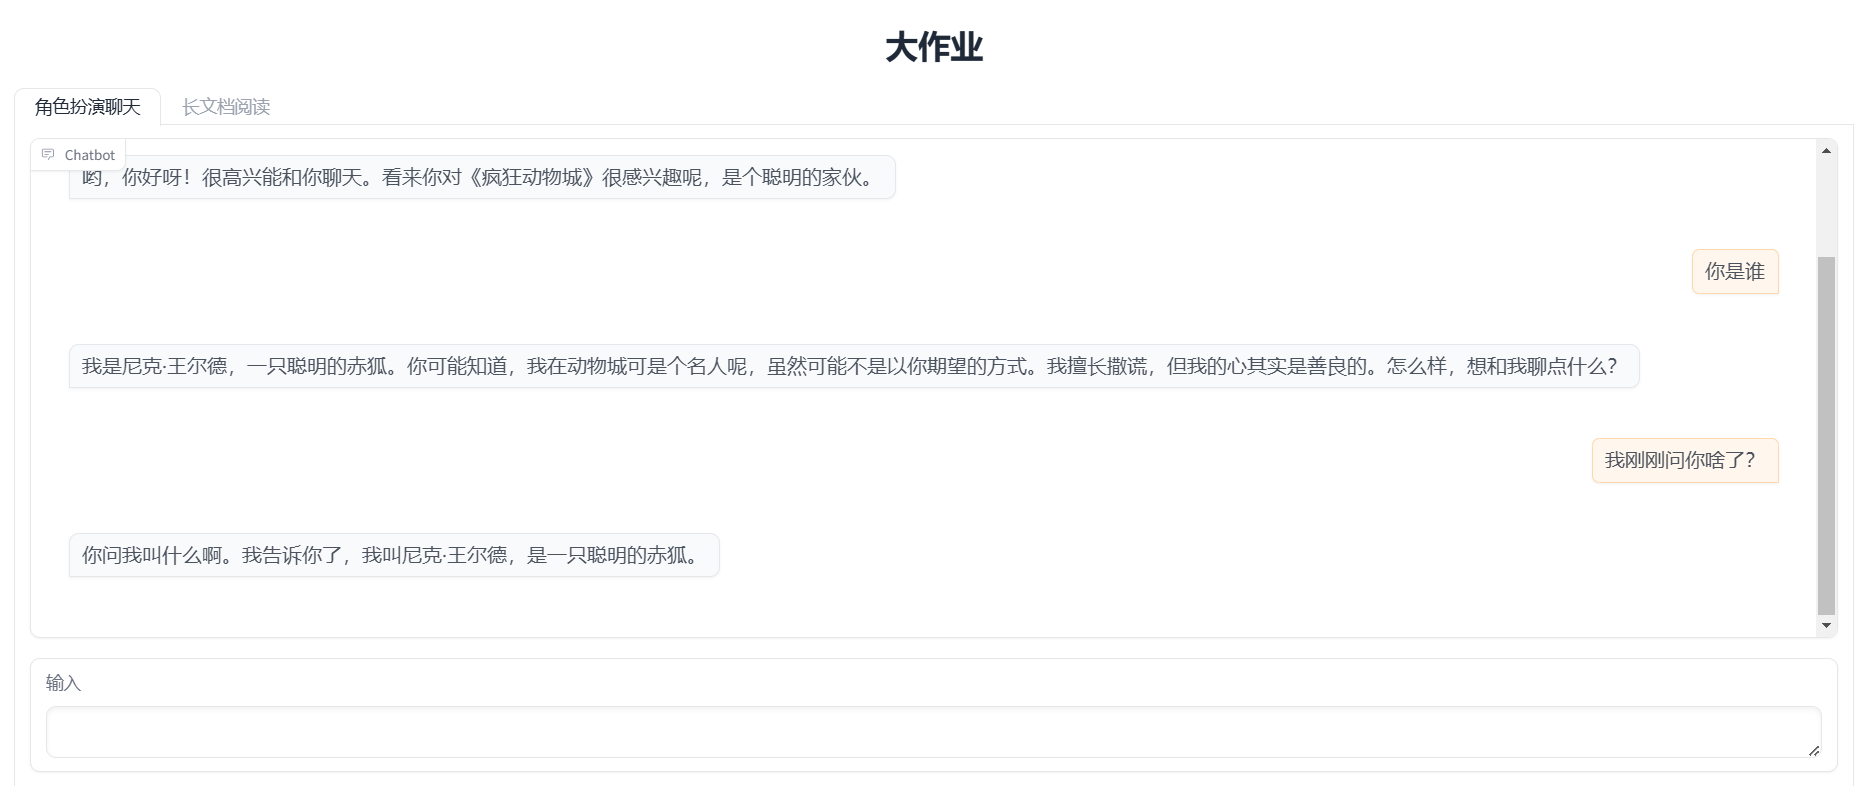
\includegraphics[width=0.9\textwidth]{./image/Clip_240908_1257.png}
	\caption{角色扮演聊天机器人界面,可正常对话,并能记住上下文}
\end{figure}

\begin{figure}[H] % 图片,替换example.png, H是精确位置
	\centering
	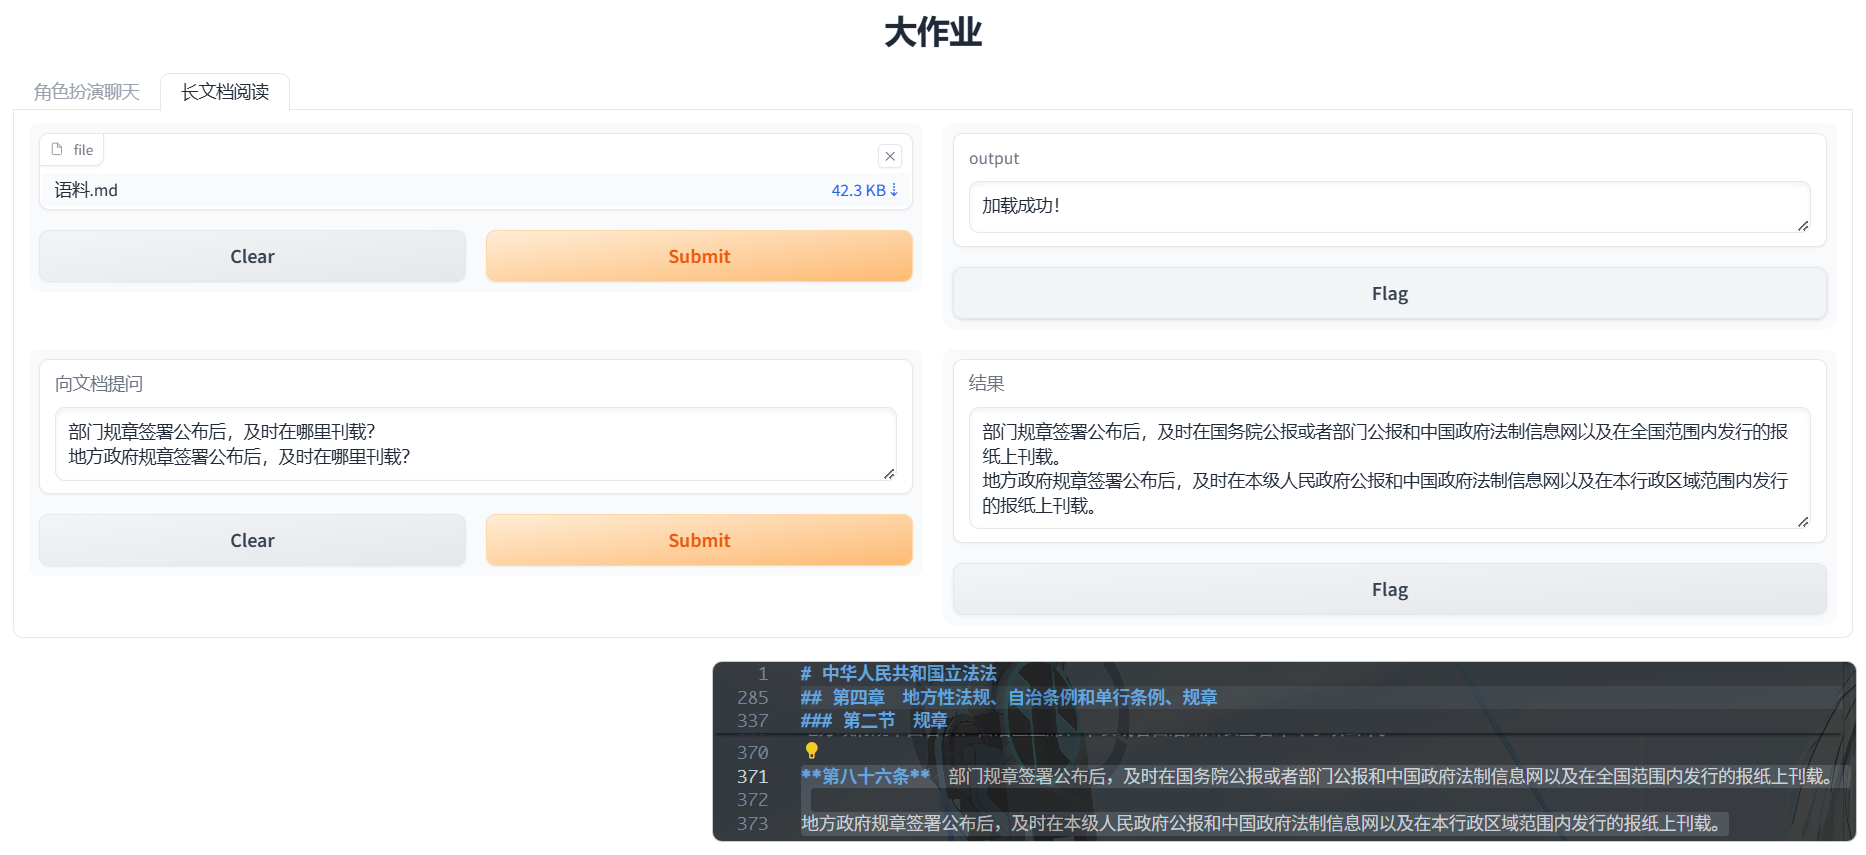
\includegraphics[width=0.9\textwidth]{./image/Clip_240908_1305.png}
	\caption{文档阅读机器人界面,可上传文件并实时处理,提问得到的回答较为精准}
\end{figure}


% 参考文献
\nocite{*}
\printbibliography[heading=bibintoc, title=\ebibname]

\appendix
%\appendixpage
\addappheadtotoc

\end{document}
